\documentclass[draftspec]{sbmlpkgspec}
\usepackage{tabularx}
\usepackage{longtable}
\usepackage{booktabs}
\usepackage{microtype}

%macros:
\newcommand{\fixttspace}{\hspace*{1pt}}

\newcommand{\sbmlthreecore}{SBML Level~3 Version~1 Core\xspace}
\newcommand{\sbmlthreedistrib}{SBML Level~3 Package Specification for Distributions, Version~1\xspace}
\newcommand{\sbmlverone}{SBML Level 3 Version 1\xspace}

\newcommand{\DrawFromDistribution}{\defRef{DrawFromDistribution}{drawFromDistribution-class}}
%\newcommand{\ExplicitPDF}{\defRef{ExplicitPDF}{explicitPDF-class}}
\newcommand{\ListOfDistribInputs}{\defRef{ListOfDistribInputs}{drawFromDistribution-class}}
\newcommand{\DistribInput}{\defRef{DistribInput}{distribInput-class}}
\newcommand{\DistributionOrSample}{\defRef{DistributionOrSample}{distributionOrSample-class}}
\newcommand{\UncertML}{\defRef{UncertML}{uncertml-class}}
%\newcommand{\UncertMath}{\defRef{Math}{uncertmath-class}}
\newcommand{\Uncertainty}{\defRef{Uncertainty}{uncertainty-class}}

\newcommand{\ExplicitPMF}{\textbf{\class{ExplicitPMF}}\xspace}
\newcommand{\FluxBound}{\textbf{\class{FluxBound}}\xspace}
\newcommand{\FunctionTerm}{\textbf{\class{FunctionTerm}}\xspace}
\newcommand{\LambdaClass}{\textbf{\class{Lambda}}\xspace}
\newcommand{\ChangedMath}{\textbf{\class{ChangedMath}}\xspace}
\newcommand{\Math}{\textbf{\class{Math}}\xspace}

\newcommand{\arraysshort}{arrays\xspace}
\newcommand{\arrays}{Arrays\xspace}
\newcommand{\distribshort}{\emph{distrib}\xspace}
\newcommand{\distrib}{Distributions\xspace}
\newcommand{\mathml}{MathML\xspace}
\newcommand{\req}{Required Elements\xspace}
\newcommand{\uncertml}{UncertML\xspace}

\reversemarginpar  % Want "\watchout" to be put on the left, not the right.
\newcommand{\watchout}{\marginpar{\hspace*{34pt}\raisebox{-0.5ex}{\Large\ding{43}}}}
\newcommand{\controversial}{\marginpar{\hspace*{34pt}\raisebox{-0.5ex}{\Large?}}}

\begin{document}

\packageTitle{The Distributions Package\\for SBML Level 3}
\packageVersion{Version 0.12 (Draft)}
\packageVersionDate{XX June, 2013}
%\packageGeneralURL{http://sbml.org/Community/Wiki/SBML_Level_3_Proposals/Distributions_and_Ranges}
%\packageThisVersionURL{}

\author{%
  \begin{tabular}{c>{\hspace{20pt}}c}
    \multicolumn{2}{c}{\Large\bf{Authors}}\\\\
    Stuart L Moodie                     & Lucian P Smith\\
    \mailto{moodie@ebi.ac.uk}           & \mailto{lpsmith@uw.edu}\\
    EMBL-EBI                            & California Institute of Technology\\
    Hinxton, UK                         & Seattle, WA, USA\\
  \\
    \multicolumn{2}{c}{\Large\bf{Contributors}}\\\\
    Nicolas Le Nov\`{e}re               & Darren Wilkinson\\
    \mailto{lenov@babraham.ac.uk}       & \mailto{darren.wilkinson@ncl.ac.uk}\\
    Babraham Institute                  & University of Newcastle\\
    Babraham, UK                        & Newcastle, UK\\
  \\
    Maciej Swat                         & Sarah Keating\\
    \mailto{mjswat@ebi.ac.uk}           & \mailto{skeating@ebi.ac.uk}\\
    EMBL-EBI                            & EMBL-EBI\\
    Hinxton, UK                         & Hinxton, UK\\
\\
     \multicolumn{2}{c}{ Colin Gillespie}\\
     \multicolumn{2}{c}{\mailto{c.gillespie@ncl.ac.uk}}\\
     \multicolumn{2}{c}{University of Newcastle}\\
     \multicolumn{2}{c}{ Newcastle, UK}\\
\end{tabular}
}

\frontNotice{Disclaimer: This is a working draft of the SBML Level 3
  ``distib'' package proposal. It is not a normative document.  Please
  send comments and other feedback to the mailing list:
  \mailto{sbml-distrib@lists.sourceforge.net.}}

\maketitlepage
\maketableofcontents

\section*{Revision History}

\begin{edtable}{tabularx}{\linewidth}{c c c X }\toprule
\textbf{Version} & \textbf{Date} & \textbf{Author} & \textbf{Comments} \\ \midrule
0.1 (Draft) & 15 Oct 2011 & Stuart Moodie & First draft \\ \midrule
0.2 (Draft) & 16 Oct 2011 & Stuart Moodie & Added introductory text
and background info. Other minor changes etc. \\ \midrule
0.3 (Draft) & 16 Oct 2011 & Stuart Moodie & Filled empty invocation
semantics section.\\ \midrule
0.4 (Draft) & 4 Jan 2012 & Stuart Moodie & Incorporated comments from
NlN, MS and SK. Some minor revisions and corrections.\\  \midrule
0.5 (Draft) & 6 Jan 2012 & Stuart Moodie & Incorporated addition
comments on aim of package from NlN.\\ \midrule
0.6 (Draft) & 19 Jul 2012 & Stuart Moodie & Incorporated revisions
discussed and agreed at HARMONY 2012.\\ \midrule
0.7 (Draft) & 6 Aug 2012 & Stuart Moodie & Incorporated review
comments from Maciej Swat and Sarah Keating.\\ \midrule
0.8 (Draft) & 21 Dec 2012 & Stuart Moodie & Incorporated changes
suggested at combine and subsequently through list discussions.\\ \midrule
0.9 (Draft) & 9 Jan 2013 & Stuart Moodie & Incorporated corrections
and comments from Maciej Swat and Sarah Keating.\\ \midrule
0.10 (Draft) & 10 Jan 2013 & Stuart Moodie & Modified based on comments
from MS.\\ \midrule
0.11 (Draft) & 17 May 2013 & Lucian Smith & Modified based on Stuart's proposals and PWG discussion.\\ \midrule
0.12 (Draft) & XX June 2013 & Lucian Smith and Stuart Moodie & Modified based on HARMONY 2013 discussion.\\
\bottomrule
\end{edtable}

\section{Introduction and motivation}

\subsection{What is it?}

The \distrib package (also affectionately known as \distribshort for
short) provides an extension to SBML Level 3 that enables a model to encode and sample from
both discrete and continuous probability distributions, and provide
the ability to annotate elements with information about the distribution their
values were drawn from. 
Applications of the package include for instance descriptions of
population based models: an important subset of which are
pharmacokinetic/pharmacodynamic (PK/PD) models\footnote{for more
  information see: \url{http://www.pharmpk.com/}.}, which are used to
model the action of drugs.

Note that originally the package was called Distributions and Ranges,
but Ranges and the use of probability distributions to describe
statistical uncertainly are no longer in the scope, hence the name change.

\subsection{Scope}

The \distrib package adds support to SBML for sampling from a
probability distribution. In particular the following are in scope:

\begin{itemize}
\item Sampling from a continuous distribution.
\item Sampling from a discrete distribution.
\item Sampling from user-defined discrete probability density function.
\item The specification of descriptive statistics (mean, standard
  deviation, standard error, etc.).
\end{itemize}

At one point the following were considered for inclusion in this
package but are now \textbf{out of scope}:

\begin{itemize}
\item Sampling from user-defined probability density function.
\item Stochastic differential equations.
\item Other functions used to characterise a probability distribution,
  such as cumulative distribution functions (CDF) or survival functions, etc.
\end{itemize}

\subsection{This Document}

This proposal describes the consensus view of workshop participants
and subscribers to the sbml-distrib mailing list. Although it was
written by the listed authors it does not soley reflect their views nor is
it their proposal. Rather, it is their understanding of the consensus
view of what the \distrib package should do and how it should do
it. The contributors listed have made significant contributions to the
development and writing of this specification and are credited
accordingly, but a more comprehensive attribution is provided in the
acknowledgements (\sec{sec:acknowledgements}).

Finally, there are issues that have arisen during the writing of this
document (\ref{sec:unresolved}). It is important that they are
considered and resolved and so the author(s) would encourage the
reader to consider them and contribute their ideas or comments ---
indeed any feedback about this proposal --- to the \distribshort
discussion list\footnote{\mailto{sbml-distrib@lists.sourceforge.net}}.

Once the proposal is finalised this will be the first step towards the
formal adoption of the \distribshort as a package in SBML Level
3. After this, two implementations based on this proposal are required
and then a vote on its adoption by the SBML community. The proposal
will then provide the basis for a future package specification
document. More details of the SBML package adoption process can be
found at: \url{http://sbml.org/Documents/SBML_Development_Process}.


\subsection{Conventions used in this document}

As we are early in the package proposal process there will be some
parts of this proposal where there is no clear consensus on the
correct solution or only recent agreement or agreement by a group
which may not be representative of the SBML community as a
whole. These cases are indicated by the \controversial question mark
in the left margin (illustrated). The reader should pay particular
attention to these points and ideally provide feedback, especially if
they disagree with what is proposed. Similarly there will be points
--- especially as the proposal is consolidated --- which are agreed,
but which the reader should take note of and perhaps read again. These
points \watchout are emphasised by the hand pointer in the left margin
(illustrated).

\section{Background}

\subsection{Problems with current SBML approaches}

SBML Level 3 Core has no direct support for encoding random values
within a model. Currently there is no workaround within the core
language itself, although it is possible to define such information
using annotations within SBML itself. Frank Bergmann had proposed such
an semi-formalised extension for use with SBML L2 [REF?].

\subsection{Past work on this problem or similar topics}

\subsubsection{The Newcastle Proposal}
\label{sec:newcastle proposal}

In 2005 there was a proposal from Colin Gillespie and others
\footnote{\url{http://sbml.org/Community/Wiki/SBML\_Leve\l_3\_Proposals/Distributions\_and\_Ranges}}
to introduce support for probability distributions in the SBML core specification. This
was based on their need to use such distributions to represent the
models they were creating as part of the BASIS project
(\url{http://www.basis.ncl.ac.uk}).

They proposed that distributions could be referred to in SBML using
the \class{csymbol} element in the \mathml subset used by
the SBML Core specification. An example is below:

\begin{example}
<xmlns=''http://www.w3.org/1998/Math/MathML''>
  <apply>
    <csymbol encoding=''text''
        definitionURL=''http://www.sbml.org/sbml/symbols/uniformRandom''>
      uniformRandom
    </csymbol>
    <ci>mu</ci>
    <ci>sigma</ci>
  </apply>
</math>
\end{example}

This required that a library of definitions be maintained as part of
the SBML standard and in their proposal they defined an initial small
set of commonly used distributions. The proposal was never
implemented.

\subsubsection{Seattle 2010}

The ``distrib'' package was discussed at the Seattle SBML Hackathon%
\footnote{\url{http://sbml.org/Events/Hackathons/The_2010_SBML-BioModels.net_Hackathon}}
and this section is an almost verbatim reproduction of Darren
Wilkinson's report on the
meeting\footnote{\url{http://sbml.org/Forums/index.php?t=tree\&goto=6141\&rid=0}}. There
Darren presented an overview of the problem%
\footnote{Slides: \url{http://sbml.org/images/3/3b/Djw-sbml-hackathon-2010-05-04.pdf}}%
\footnote{Audio: \url{http://sbml.org/images/6/67/Wilkinson-distributions-2010-05-04.mov}},
building on the old proposal from the Newcastle group (see above:
\ref{sec:newcastle proposal}).  There was broad support at the meeting
for development of such a package, and for the proposed feature
set. Discussion following the presentation led to a consensus on the
following points:

\begin{itemize}
\item There is an urgent need for such a package.
\item It is important to make a distinction between a description of
  uncertainty regarding a model parameter and the mechanistic process
  of selecting a random number from a probability distribution, for
  applications such as parameter scans and experimental design
\item It is probably worth including the definition of PMFs, PDFs and CDFs in the package
\item It is worth including the definition of random distributions using particle representations within such a package, though some work
 still needs to be done on the precise representation
\item It could be worth exploring the use of xinclude to point at particle
representations held in a separate file
\item Random numbers must not be used in rate laws or anywhere else that
 is continuously evaluated, as then simulation behaviour is not
 defined
\item Although there is a need for a package for describing extrinsic
 noise via stochastic differential equations in SBML, such mechanisms
 should not be included in this package due to the considerable
 implications for simulator developers
\item We probably don't want to layer on top of \uncertml
 (www.uncertml.org), as this spec is fairly heavy-weight, and
 somewhat tangential to our requirements
\item A random number seed is not part of a model and should not be
 included in the package
\item The definition of truncated distributions and the specification of
 hard upper and lower bounds on random quantities should be
 considered.
\end{itemize}

It was suggested that new constructs should be introduced into SBML by
the package embedded as user-defined functions using the following
syntax:

\begin{example}
<listOfFunctionDefinitions>
  <functionDefinition id="myNormRand">
    <distrib:####>
      #### distrib binding information here ####
    </distrib:####>
    <math>
      <lambda>
        <bvar>
          <ci>mu</ci>
          <ci>sigma</ci>
        </bvar>
        <ci>mu</ci>
      </lambda>
    </math>
  </functionDefinition>
</listOfFunctionDefinitions>
\end{example}

which allows the use of a "default value" by simulators which do not
understand the package (but simulators which do will ignore the <math>
element). The package would nevertheless be "required", as it will not
be simulated correctly by software which does not understand the
package.

Informal discussions following the break-out covered topics such as:

\begin{itemize}
\item how to work with vector random quantities in the absence of the vector
element in the MathML subset used by SBML
\item how care must be taken with the semantics of random variables
  and the need to both:
\begin{itemize}
\item reference multiple independent random quantities at a given
  time
\item make multiple references to the same random quantity at a given
time.
\end{itemize}
\end{itemize}

\subsubsection{Hinxton 2011}

Detailed discussion was continued at the Statistical Models Workshop
in Hinxton in June 2011%
\footnote{\url{http://sbml.org/Events/Other_Events/statistical_models_workshop_2011}}. There
those interested in representing Statistical Models in SBML came
together to work out the details of how this package would work in
detail. Dan Cornford from the \uncertml
project\footnote{\url{http://www.uncertml.org/}} attended the meeting
and described how that resource could be used to describe uncertainty
and in particular probability distributions. Perhaps the most
significant decision at this meeting was to adopt the \uncertml
resource as a controlled vocabulary that is referenced by the \distrib package.

Much has changed since this meeting, but the output from this meeting
was the basis for the first version of this proposal.


\subsubsection{HARMONY 2012: Maastricht}

Two sessions were dedicated to discussion of \distrib at HARMONY based
around the proposals described in version 0.5 of this document. In
addition there was discussion about the \arrays proposal which was
very helpful in solving the problem of multivariate distributions in
\distrib. The following were the agreed outcomes of the meeting:

\begin{itemize}
\item The original proposal included UncertML markup directly in the
  function definition. This proved unwieldy and confusing and has been
  replaced by a more elegant solution that eliminates the UncertML
  markup and integrates well with the fallback function (see details
  below).
\item Multivariate distributions can be supported using the \arrays
  package to define a covariance matrix.
\item User defined continuous distributions would define a PDF in
  \mathml.
\item Usage semantics were clarified so that invokation of a function
  definition implied a value was sampled from the specified
  distribution.
\item It was agreed from which sections of an SBML model a
  distribution could be invoked.
\item Statistical descriptors of variables (for
  example mean and standard deviation) would be separated from
  \distrib and either provided in a new package or in a later version
  of SBML L3 core.
\end{itemize}

\subsubsection{COMBINE 2012: Toronto}

The August proposal was reviewed and an improvement was agreed to
the user-defined PMF part of the proposal. In particular is was agreed
that the categories should be defined by \distribshort classes rather
than by passing in the information as an array. Questions were also raised
about whether \uncertml was suitably well defined to be used as an
external definition for probability distributions. This was resolved
subsequent to the meeting with a teleconference to Dan Cornford and
colleagues. These changes are incorporated here. Finally, there was
considerable debate about whether to keep the dependence of
\distribshort on the Arrays package in order to support multi-variate
distributions. The outcome was an agreement that we would review this
at the end of 2012, based on the results of an investigation
into how feasible it would be to implement \arrays as a package.

\subsubsection{2013 Package Working Group discussions}

Early 2013 saw a good amount of discussion on the \distribshort Package Working Group mailing list, spurred by proposals by Stuart Moodie\footnote{\url{http://thestupott.wordpress.com/2013/03/12/an-improved-distrib-proposal/}}.  While not all of his suggestions ended up being fully accepted by the group, several changes were accepted, including:

\begin{itemize}
\item To use UncertML as actual XML, instead of as a set of reference definitions.
\item To use UncertML to encode descriptive statistics of SBML elements such as mean, standard deviation, standard error, etc.) bringing this capability back in scope for this package.
\end{itemize}


\subsubsection{HARMONY 2013: Connecticut}

At HARMONY at UConn in Connecticut, further discussions revealed the importance of distinguishing the ability to describe an element as a distributed variable vs. a function call within the model performing a draw from a distribution.

We also decided to discard the encoding of explicit PDFs for now, as
support for it is remarkably complicated, and there no demand for
it. The current design could be extended to support this feature so if
there is demand for it in the future support for explicit PDFs could
be reintroduced.

\section{Proposed syntax and semantics}

\subsection{Overview}

Following the precedent set by the SBML Level~3 Core specification
document, we use UML~1.0 (Unified Modeling Language;
\citealt{eriksson:1998,oestereich:1999}) class diagram notation to
define the constructs provided by this package.  We also use color in
the diagrams to carry additional information for the benefit of those
viewing the document on media that can display color.  The following are
the colors we use and what they represent:

\begin{itemize}

\item[\raisebox{2.75pt}{\colorbox{black}{\rule{0.8pt}{0.8pt}}}]
  \emph{Black}: Items colored black in the UML diagrams are components
  taken unchanged from their definition in the SBML Level~3 Core
  specification document.

\item[\raisebox{2.75pt}{\colorbox{mediumgreen}{\rule{0.8pt}{0.8pt}}}]
  \emph{\textcolor{mediumgreen}{Green}}: Items colored green are
  components that exist in SBML Level~3 Core, but are extended by this
  package.  Class boxes are also drawn with dashed lines to further
  distinguish them.

\item[\raisebox{2.75pt}{\colorbox{darkblue}{\rule{0.8pt}{0.8pt}}}]
  \emph{\textcolor{darkblue}{Blue}}: Items colored blue are new
  components introduced in this package specification.  They have no
  equivalent in the SBML Level~3 Core specification.

\end{itemize}

We also use the following typographical conventions to distinguish the
names of objects and data types from other entities; these conventions
are identical to the conventions used in the SBML Level~3 Core specification
document:

\begin{description}
  
\item \abstractclass{AbstractClass}: Abstract classes are never
  instantiated directly, but rather serve as parents of other classes.
  Their names begin with a capital letter and they are printed in a
  slanted, bold, sans-serif typeface.  In electronic document formats,
  the class names defined within this document are also hyperlinked to
  their definitions; clicking on these items will, given appropriate
  software, switch the view to the section in this document containing
  the definition of that class.  (However, for classes that are
  unchanged from their definitions in SBML Level~3 Core, the class names
  are not hyperlinked because they are not defined within this
  document.)
  
\item \class{Class}: Names of ordinary (concrete) classes begin with a
  capital letter and are printed in an upright, bold, sans-serif
  typeface.  In electronic document formats, the class names are also
  hyperlinked to their definitions in this specification document.
  (However, as in the previous case, class names are not hyperlinked if
  they are for classes that are unchanged from their definitions in the
  SBML Level~3 Core specification.)

\item \token{SomeThing}, \token{otherThing}: Attributes of classes, data
  type names, literal XML, and tokens \emph{other} than SBML class
  names, are printed in an upright typewriter typeface.  Primitive types
  defined by SBML begin with a capital letter; SBML also makes use of
  primitive types defined by XML
  Schema~1.0~\citep{biron:2000,fallside:2000,thompson:2000}, but
  unfortunately, XML~Schema does not follow any capitalization
  convention and primitive types drawn from the XML~Schema language may
  or may not start with a capital letter.

\end{description}

For other matters involving the use of UML and XML, we follow the
conventions used in the SBML Level~3 Core specification document.  


\subsection{Namespace URI and other declarations necessary for using this package}
\label{xml-namespace}

Every SBML Level~3 package is identified uniquely by an XML namespace URI.  For an SBML document to be able to use a given Level~3 package, it must declare the use of that package by referencing its URI.  The following is the namespace URI for this version of the \distrib package for \sbmlthreecore:
\begin{center}
\uri{http://www.sbml.org/sbml/level3/version1/distrib/version1}
\end{center}

In addition, SBML documents using a given package must indicate whether the package may be used to change the mathematical meaning of \sbmlthreecore elements.  This is done using the attribute \token{required} on the \token{<sbml>} element in the SBML document.  For the \distrib package, the value of this attribute must be \val{true}, as the \DrawFromDistribution element overrides the core definition of a \FunctionDefinition.  Note that the value of this attribute must \emph{always} be set to \val{true}, even if the particular model does not contain any \DrawFromDistribution elements.

The following fragment illustrates the beginning of a typical SBML model using \sbmlthreecore and this version of the \distrib package:

\begin{example}
<?xml version="1.0" encoding="UTF-8"?>
<sbml xmlns="http://www.sbml.org/sbml/level3/version1/core" level="3" version="1"
      xmlns:distrib="http://www.sbml.org/sbml/level3/version1/distrib/version1"
      distrib:required="true">
\end{example}


\subsection{Primitive data types}
\label{new-primitive-types}

The \distrib package uses the \val{string} primitive data type described in Section~3.1 of the \sbmlthreecore specification, and adds two additional primitive types described below.


\subsubsection{Type \fixttspace\primtypeNC{UncertId}}
\label{primtype-portid}

The type \primtype{UncertId} is derived from \primtype{SId} (\sbmlthreecore specification Section~3.1.7) and has identical syntax.  The \primtype{UncertId} type is used to create local IDs that can be used in the extended \FunctionDefinition objects to refer to the arguments of the function, in much the same way that the identities of the \token{bvar} elements are used in MathML \token{lambda} elements.  Each \primtype{UncertId} has a scope local to the \DrawFromDistribution in which it is found.  The
equality of \primtype{UncertId} values is determined by an exact
character sequence match; i.e., comparisons of these identifiers must be
performed in a case-sensitive manner.


\subsubsection{Type \fixttspace\primtypeNC{UncertIdRef}}
\label{primtype-portidref}

Type \primtype{UncertIdRef} is used for references to
identifiers of type \primtype{UncertId}.  This type is derived from
\primtype{UncertId}, but with the restriction that the value of an
attribute having type \primtype{UncertIdRef} must match the value of a
\primtype{UncertId} found in the same parent \DrawFromDistribution as the
\primtype{UncertIdRef}.  As with \primtype{UncertId}, the equality of
\primtype{UncertIdRef} values is determined by exact character sequence
match; i.e., comparisons of these identifiers must be performed in a
case-sensitive manner.



\subsection{Defining Distributions}

\subsubsection{The approach}

The \distrib package has two very simple purposes. First, it provides a
mechanism for sampling a random value from a probability
distribution. This implies that it must define the probability distribution and then must sample a
random value from that distribution.

Secondly, it provides a mechanism for describing elements with information about their uncertainty.  One common use case for this will be to provide the standard deviation for a value.  Another may be describing a parameter's distribution, so that a better search can be performed in a parameter scan experiment.

Both purposes are achieved by using \uncertml.  Probability density functions (PDFs) are defined in the \val{Distri\-butions} branch of \uncertml, probability mass functions (PMFs) are defined in the \val{Samples} branch, and summary statistics in the \val{Statistics} branch.

%The second way is to define
%a probability density function (PDF) using MathML.

It is technically possible to provide an explicit PDF in MathML instead of using the pre-defined PDFs from \uncertml.  However, one advantage of using the UncertML pre-defined
distributions is that software can easily recognise the distribution
and use an optimised built-in implementation rather than interpreting
the distribution from the PDF definitions. For some
applications such optimisations make important performance
differences.  Another advantage is that some software may only support certain types of distributions, and having them predefined makes it simpler for the software to inform a user that a particular distribution is not supported.

It is hoped that if users find the need to define distributions not covered by UncertML, that they will either be able to encode those distributions as combinations of other predefined distributions, or that they will be able to persuade \uncertml to either add the new distribution to the list.

When a distribution is defined in a \FunctionDefinition, it is sampled when it is invoked. To reuse a
sampled value, the value must be assigned to a parameter first, such as through the use of an \InitialAssignment or \EventAssignment.  When a distribution is defined elsewhere, that information may be used outside of the model, using whatever methodology is appropriate to answer the question being pursued.


\subsection{The extended \class{FunctionDefinition} class}

To model random processes, this package extends the \FunctionDefinition class as
can be seen in the UML representation in \fig{fig:funcdef}. The redefined \FunctionDefinition optionally
contains a single \token{drawFromDistribution} child.

The \FunctionDefinition class must still contain the
\mathml block containing the standard SBML function definition. This is
required to comply with the \emph{Validity after Reduction} rule in the
package design guidelines \cite{sbmll3v1packrule} and ensures a degree
of backwards compatibility for SBML readers and validators that do not
understand the \distribshort package.

\begin{figure}[htb]
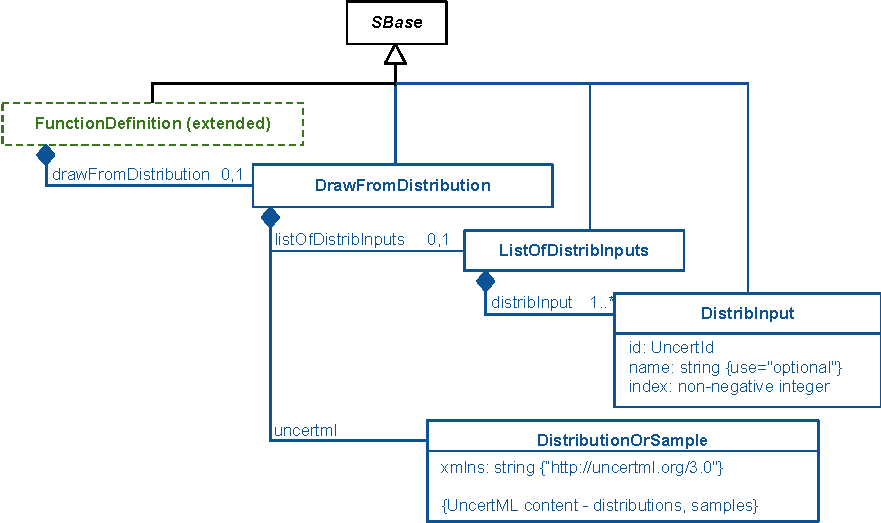
\includegraphics[width=0.75\linewidth]{distrib-functionDefinition.pdf}
\caption{The definition of the extended \FunctionDefinition class, plus the \DrawFromDistribution, \ListOfDistribInputs, \DistribInput, and \DistributionOrSample classes.  A \DrawFromDistribution element must have exactly one \DistributionOrSample child.  Together, these classes provide a way to transform a \FunctionDefinition to sample from a probability density function or a probability mass function.}
\label{fig:funcdef}
\end{figure}


As outlined above, the \FunctionDefinition class is extended to contain a \DrawFromDistribution child.  Because a \FunctionDefinition must have a \LambdaClass child according to \sbmlthreecore, a valid function will still have one, but the \token{drawFromDistribution} child, if present, will override any definition found there.  However, software that does not support \distribshort could potentially invoke the function found in the \LambdaClass element (see \ref{sec:fallbackfunc}).

In the \Model, an extended \FunctionDefinition may be used in any \mathml to perform a draw from a distribution.  This draw will be unique for every use of the \FunctionDefinition, whether or not the draw is performed at the same simulation time as a different draw (for example, if used in two different \InitialAssignment elements).

%In the \Model, an extended \FunctionDefinition can have two different uses.  First, it may be used in any \mathml to perform a draw from a distribution.  This draw will be unique for every use of the \FunctionDefinition, whether or not the draw is performed at the same simulation time as a different draw (for example, if used in two different \InitialAssignment elements).

%Secondly, it may be used in an \Uncertainty element to denote that a particular element has the uncertainty defined by the extended function.  See \sec{uncertmath-class} for more details.



\subsection{The \class{DrawFromDistribution} class}
\label{drawFromDistribution-class}

As illustrated in \fig{fig:funcdef}, the \DrawFromDistribution class may have a \ListOfDistribInputs child, which must in turn contain one or more \DistribInput children, which act as the arguments to the function--they serve the same role as the \token{bvar} elements of the \LambdaClass child of a \FunctionDefinition.  The order of arguments is determined by the \token{index} attribute:  the first argument (if any) must have an index of \val{0}, the second of \val{1}, etc.

It must also have a \DistributionOrSample child, representing a probability density function (PDF) or probability mass function (PMF) defined by \uncertml.  Within the \uncertml, the \primtype{UncertId}s defined by the \DistribInput objects are used as the variables within the distribution.


\subsection{The \class{DistribInput} class}
\label{distribInput-class}

The \DistribInput class mimics the \token{bvar} elements of MathML lambda functions.  It must have an \token{id} attribute of type \primtype{UncertId} and an \token{index} attribute of type \primtype{non-negative integer}.  It may additionally have a \token{name} attribute of type \token{string}, which may be used in the same manner as other \token{name} attributes on \sbmlthreecore objects; please see Section~3.3.2 of the \sbmlthreecore specification for more information.

Each \DistribInput element represents an argument to the function, and serves as a local identifier, referenced only by the \uncertml in the sibling \DistributionOrSample class. See the examples in \ref{sec:fd-examples} for more details.

Because the \LambdaClass child of the \FunctionDefinition is required, it must have the same number of \token{bvar} children as the \DrawFromDistribution has \DistribInput children.  They do not, however, have to have the same IDs:  the \token{bvar} ids are defined as being local to the \LambdaClass function in much the same way that the \DistribInput IDs are defined as being local to the \DrawFromDistribution object.

Each \token{index} attribute on a \DistribInput within a \ListOfDistribInputs element must have a unique value, numbered consecutively from \val{0}:  if one \DistribInput is present, its \token{index} value must be \val{0}; if there are two, they must have \token{index} values of \val{0} and \val{1}, etc.

%The value \val{x} may not be used as an \primtype{UncertId} in an \DistribInput element; that symbol is reserved for use by the \ExplicitPDF element (see \ref{explicitPDF-class}).

\subsection{The \class{DistributionOrSample} class}
\label{distributionOrSample-class}

The \DistributionOrSample class, like the \Math class of many \sbmlthreecore elements, is a container for UncertML XML.  It must contain one of the 28 'Distribution' elements or one of the three 'Samples' elements (RandomSample, SystematicSample, or UnknownSample) defined at \url{http://uncertml.org/dictionary}, and have the namespace \val{http://uncertml.org/3.0}.  Note that as of this writing, UncertML is only formally defined through version 2.0, making this use of version 3.0 somewhat speculative.  However, the \distribshort Package Working Group has been in communication with the developers of UncertML, and feel certain that the change needed in UncertML to accomodate its use in this package (namely, the possible substitution of IDs for numbers) will be made for UncertML 3.0.

When a \DistributionOrSample is encountered, its parent \FunctionDefinition is defined as sampling from the defined distribution, and returning that sample.  It may contain any number of \token{UncertIdRef} strings, each of which must correspond to an \token{UncertId} defined in a \DistribInput in the same function.

The full list of the 28 distributions and how they can be used is provided in \ref{sec:uncertmlusage}.  Four of these distributions (Dirichlet, Multinomial, Multivariate Normal, and Multivariate Student T) use vectors as both input and output.  It is possible, if tedious, to provide vector input to these distributions by simply defining each element of the required vector as a numeric value or as an \primtype{UncertId}.  However, it is not possible in \sbmlthreecore to take a single vector and simultaneously assign its values to different elements, or even to use a vector within MathML.  While it would be theoretically possible to define new elements in this specification to work around this limitation, such capabilities are more obviously the domain of the Arrays package within SBML, or of SED-ML\footnote{\url{http://sed-ml.org/}} (to set a suite of element values).  Unfortunately, as of this writing, the Arrays package has not yet been finalized, and many aspects of it have not been set.  Therefore, it is left to the future finalized Arrays package to define how to utilize a \FunctionDefinition that returns a vector, and how to define a \FunctionDefinition that takes a vector as input.  It is also possible for other individuals or groups to come up with custom annotations that define how to do this, and in fact, this is encouraged for any group that requires the use of any of these four distributions for their models.  If no such definitions exist, however, any numerical results from the use of these functions remain undefined, and models using this technique are unsimulatable.  (Such models may still be useful descriptions of certain situations, however.)  A final possibility is that SED-ML could be extended to extract the function definition, perform the sampling itself, and use the resulting vector to assign initial values to certain elements.

All three Sample elements in UncertML are logistically identical, and only semantically different.  The RandomSample describes a set of realizations known to come from a randomly-distributed source.  The SystematicSample describes a set of deliberately chosen realizations, such as those resulting from unscented sampling methods for Gaussian random variables.  The UnknownSample describes a set of realizations for which the source distribution is unknown.  All three describe a set of realizations, each with a weight and one or more values. The weights of all realizations in a single Sample must sum to 1.0.

UncertML also allows the definition of realizations with \val{categories} instead of \val{values} (i.e. \primtype{strings} instead of \primtype{doubles}).  This data type is unsupported in\sbmlthreecore, but if a package supports this data type in the future (as the Qualitative Models package might), \val{categories} could be used.

When a \DistributionOrSample is encountered containing a Sample, its parent \FunctionDefinition is defined as randomly choosing a single realization from the the \uncertml according to its \token{weight}, and, if the realization contains a \token{values} child, returning that value (or vector of values) when the function is called.  If the realization contains a \token{categories} child, that string (or vector of strings) is returned instead.  (\uncertml requires that a single realization contain either a \token{values} or \token{categories} child, but may not have both.)

As happens with some of the UncertML distributions above, then, if the chosen realization has multiple values or categories, the result of the draw is a vector, which cannot, in \sbmlthreecore, be used either in MathML or as an assignment to an SBML element.  The Arrays package or some form of custom annotation must be used to define what happens when a multi-value realization is chosen.

Similarly, there is no \token{string} data type for SBML elements defined in \sbmlthreecore.  Without a package that defines such a data type, then, any call to a \FunctionDefinition that returns a string or vector of strings from a \token{categories} \uncertml element will be undefined and therefore unsimulatable, but may, again, be a useful description of a particular type of model.

Note \notice that the \ExplicitPMF class in previous versions of this specification did not use \uncertml, and instead defined its own way of listing samples.  The functionality (with the addition of IDs instead of numbers in \uncertml 3.0) is identical.


%\subsection{The \class{ExplicitPDF} class}
%\label{explicitPDF-class}

%The \ExplicitPDF class is a container for MathML XML.  It must define a function, using the same MathML allowed in the rest of the SBML Document, for the value \val{x} that integrates to 1.0 over all \token{x}, and which never evaluates to a negative value for any \token{x}.  It may also use the \primtype{UncertIDRef} identifiers defined by its sibling \DistribInput elements, and the \primtype{SId}s of any other \FunctionDefinition, but no other identifier.  For this reason, \val{x} is illegal to use as an \primtype{UncertId} in any \DistribInput element in the model:  it is reserved for use by the \ExplicitPDF class.  As is the case in \sbmlthreecore, circular function definitions are illegal: the \primtype{SId} of a \FunctionDefinition may not be used in its own child \ExplicitPDF, nor may it use the \primtype{SId} of a \FunctionDefinition that references itself, etc.


\subsection{Discrete vs. continuous sampling}
\label{discrete-continuous}

The \primtype{SId}s of \FunctionDefinition elements can be used in \sbmlthreecore in both discrete and continuous contexts:  \InitialAssignment, \EventAssignment, \Priority, and \Delay elements are all discrete, while \Rule, \KineticLaw, and \Trigger elements are all continuous in time.  For discrete contexts, the behavior of \distribshort-extended \FunctionDefinition elements is well-defined:  one or more random values are sampled from the distribution each time the function definition is invoked. Each invocation implies one sampling operation.  In continuous contexts, however, their behavior is ill-defined.  More information than is defined in this package (such as autocorrelation values or full conditional probabilities) would be required to make random sampling tractable in continuous contexts, and is beyond the scope of this version of the package.  If some package is defined in the future that adds this information, or if custom annotations are provided that add this information, such models may become simulatable.  However, this package does not define how to handle sampling in continuous contexts, and recommends against it: a warning may be produced by any software encountering the use of a \distribshort-extended \FunctionDefinition in a continuous context.  Assuming such models are desirable, and the information is not provided in a separate package, this information may be incorporated into a future version of this specification.

Any other package that defines new contexts for MathML will also either be discrete or continuous.  Discrete situations (such as those defined in the Qualitative Models package) are, as above, well-defined.  Continuous situations (as might arise within the Spatial Processes package, over space instead of over time) will most likely be ill-defined.  Those packages must therefore either define for themselves how to handle \distribshort-extended \FunctionDefinition elements, or leave it to some other package/annotation scheme to define how to handle the situation.

\subsection{Truncation}
\label{truncation}

In order to perform truncation, one or both ends of the distribution are cut off, and the remaining function is re-scaled so the area under the curve is once again 1.0.  Earlier versions of this specification allowed one to specify truncation values for UncertML distributions and explicit PDFs:  upper and lower limits to the distributions, between which values must be sampled.  However, this capability is being introduced in UncertML 3.0, making truncation elements superfluous for \DistributionOrSample elements.  Truncation was never considered for inclusion for explicit PMF functions, as truncating a sample is as simple as not including the rejected realizations.  Therefore, since its capabilities are duplicated elsewhere, truncation-specific elements have been dropped from this version of the specification.

\emph{Note: \notice If the truncation elements were desired as a form of annotation, denoting the range between which most, if not all, of a given distribution would fall, that capability is not replicated in the other functions above, and would need to be re-added to this specification.}

\emph{Note 2: \notice If UncertML 3.0 doesn't actually end up having a truncation element, we can add this back in.}


\subsection{Examples using the extended \FunctionDefinition}
\label{sec:fd-examples}

Several examples are given below that illustrate various uses of an extended \FunctionDefinition.

\subsubsection{Defining and using a normal distribution with UncertML}
In the following example, a \FunctionDefinition is extended to define a draw from an UncertML-defined normal distribution:

\begin{example}
...
  <listOfFunctionDefinitions>
    <functionDefinition id="normal">
      <math xmlns="http://www.w3.org/1998/Math/MathML">
        <!-- Overridden MathML -->
      </math>
      <drawFromDistribution xmlns="http://www.sbml.org/sbml/level3/version1/distrib/version1">
        <listOfDistribInputs>
          <distribInput id="avg" index="0"/>
          <distribInput id="var" index="1"/>
        </listOfDistribInputs>
        <uncertml xmlns="http://uncertml.org/3.0">
          <NormalDistribution>
            <mean> avg </mean>
            <variance> var </variance>
          </NormalDistribution>
        </uncertml>
      </drawFromDistribution>
    </functionDefinition>
  </listOfFunctionDefinitions>
...
\end{example}

Here, the \DistribInput children of \DrawFromDistribution define the local \primtype{UncertId}s \val{avg} and \val{var}, which are then used by the \DistributionOrSample as the \token{mean} and \token{variance} of a normal distribution, as defined by UncertML.  This function could then be used anywhere the \FunctionDefinition id \val{normal} can be used, as for example in an \InitialAssignment:

\clearpage

\begin{example}
...
  <listOfInitialAssignments>
    <initialAssignment symbol="y">
      <math xmlns="http://www.w3.org/1998/Math/MathML">
        <apply>
          <ci> normal </ci>
          <ci> z </ci>
          <cn> 10 </cn>
        </apply>
      </math>
    </initialAssignment>
  </listOfInitialAssignments>
...
\end{example}

This use would apply a draw from a normal distribution with mean \val{z} and variance \val{10} to the SBML element \val{y}.

%\subsubsection{Defining a normal distribution with an explicit PDF}
%In the following example, a \FunctionDefinition is extended to define a draw from a normal distribution defined in MathML, with \val{x} as the variable to be sampled.  The normal distibution equation is described in \ref{fig:normalequation}.

%\begin{figure}[htb]
%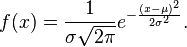
\includegraphics[width=0.2\linewidth]{gaussian_distribution_function.png}
%\caption{The equation for a normal distribution.}
%\label{fig:normalequation}
%\end{figure}


%\begin{example}
%...
%  <listOfFunctionDefinitions>
%    <functionDefinition id="normal">
%      <math xmlns="http://www.w3.org/1998/Math/MathML">
%        <!-- Overridden MathML -->
%      </math>
%      <drawFromDistribution xmlns="http://www.sbml.org/sbml/level3/version1/distrib/version1">
%         <input> mu </input>
%         <input> sigma </input>
%         <math xmlns="http://www.w3.org/1998/Math/MathML">
%            <apply>
%              <times/>
%              <apply>
%                <divide/>
%                <cn> 1 </cn>
%                <apply>
%                  <times/>
%                  <ci> sigma </ci>
%                  <apply>
%                    <root/>
%                    <degree>
%                      <cn> 2 </cn>
%                    </degree>
%                    <apply>
%                      <times/>
%                      <cn> 2 </cn>
%                      <pi/>
%                    </apply>
%                  </apply>
%                </apply>
%              </apply>
%              <apply>
%                <exp/>
%                <apply>
%                  <times/>
%                  <apply>
%                    <divide/>
%                    <apply>
%                      <power/>
%                      <apply>
%                        <minus/>
%                        <apply>
%                          <minus/>
%                          <ci> x </ci>
%                          <ci> mu </ci>
%                        </apply>
%                      </apply>
%                      <cn> 2 </cn>
%                    </apply>
%                    <cn> 2 </cn>
%                  </apply>
%                  <apply>
%                    <power/>
%                    <ci> sigma </ci>
%                    <cn> 2 </cn>
%                  </apply>
%                </apply>
%              </apply>
%            </apply>
%         </math>
%      </drawFromDistribution>
%    </functionDefinition>
%  </listOfFunctionDefinitions>
%...
%\end{example}

%Again, the \DistribInput children of \DrawFromDistribution define the local \primtype{UncertId}'s \val{mu} and \val{sigma}.  Here, they are used by the \ExplicitPDF as the \token{mean} and \token{variance} of a normal distribution of \val{x}.  This function could then be used anywhere the \FunctionDefinition id \val{normal} can be used, exactly as above.


\subsubsection{Defining a 'die roll' PMF with UncertML}
In the following example, a \FunctionDefinition is extended to define a draw from an UncertML-defined set of explicit PMFs:

\begin{example}
...
  <listOfFunctionDefinitions>
    <functionDefinition id="rolld4">
      <math xmlns="http://www.w3.org/1998/Math/MathML">
        <!-- Overridden MathML -->
      </math>
      <drawFromDistribution xmlns="http://www.sbml.org/sbml/level3/version1/distrib/version1">
         <uncertml xmlns="http://uncertml.org/3.0">
           <RandomSample>
             <Realisation>
               <weight> 0.25 </weight>
               <values> 1 </values>
             </Realisation>
             <Realisation>
               <weight> 0.25 </weight>
               <values> 2 </values>
             </Realisation>
             <Realisation>
               <weight> 0.25 </weight>
               <values> 3 </values>
             </Realisation>
             <Realisation>
               <weight> 0.25 </weight>
               <values> 4 </values>
             </Realisation>
           </RandomSample>
         </uncertml>
      </drawFromDistribution>
    </functionDefinition>
  </listOfFunctionDefinitions>
...
\end{example}

No inputs are provided.  The four \token{Realisation} children of \token{RandomSample} all have equal values for \token{weight}, and sum to 1.0, as they must.  The \token{values} of each are equally likely to be chosen, therefore, resulting in this function returning \val{1}, \val{2}, \val{3}, or \val{4}, each with equal probability.



\subsubsection{Defining a 'pick one' sample with UncertML}
In the following example, a \FunctionDefinition is extended to define a draw from an UncertML-defined set of samples:

\clearpage

\begin{example}
...
  <listOfFunctionDefinitions>
    <functionDefinition id="pickone">
      <math xmlns="http://www.w3.org/1998/Math/MathML">
        <!-- Overridden MathML -->
      </math>
      <drawFromDistribution xmlns="http://www.sbml.org/sbml/level3/version1/distrib/version1">
        <listOfDistribInputs>
          <distribInput id="A" index="0"/>
          <distribInput id="B" index="1"/>
          <distribInput id="C" index="2"/>
          <distribInput id="D" index="3"/>
        </listOfDistribInputs>
         <uncertml xmlns="http://uncertml.org/3.0">
           <RandomSample>
             <Realisation>
               <weight> 0.25 </weight>
               <values> A </values>
             </Realisation>
             <Realisation>
               <weight> 0.25 </weight>
               <values> B </values>
             </Realisation>
             <Realisation>
               <weight> 0.25 </weight>
               <values> C </values>
             </Realisation>
             <Realisation>
               <weight> 0.25 </weight>
               <values> D </values>
             </Realisation>
         </uncertml>
      </drawFromDistribution>
    </functionDefinition>
  </listOfFunctionDefinitions>
...
\end{example}

In this example, the function 'pickone' is defined, with four arguments, \val{A}, \val{B}, \val{C}, and \val{D}.  When called, each argument has an equal chance of being chosen as the return value.

{\color{red} Stuart: \controversial This seems a bit idiosyncratic to me. Are you trying to get
  round the fact that SBML doesn't support strings? If so I'd leave
  that up to the modeller. They can map numeric values to their
  categories.  }

\subsection{Equivalence with Fallback Function}
\label{sec:fallbackfunc}

The \mathml definition directly contained by the
\class{functionDefinition} is not used and is provided to
satisfy the \emph{validity after reduction} rule for packages
\cite{sbmll3v1packrule}. This rules states that the SBML document must
be syntactically valid if all package specific elements are removed
from it. To ensure that this is the case the fallback function used in
relation to \distribshort must satisfy the following rules:

\begin{itemize}
\item the lambda function should have the same number of arguments as
  its equivalent distribution (defined by \distribshort).
\item Each argument should match the type of the equivalent argument
  in the external function.
\item The lambda function should have the same return type as the
  \emph{sampled} distribution. For example, if a predefined PDF when
  sampled returns a scalar value, the dummy function should also do so.
\end{itemize}

Clearly, these rules can only be enforced by a \distribshort-aware validator.

In the following example, the fallback function is coded to simply return \val{mean}, the first argument of the function.  Note that the arguments have been given different local IDs (\val{mean} and \val{v} instead of \val{avg} and \val{var}); their equivalence is based on order, not string matching.

\clearpage

\begin{example}
  <listOfFunctionDefinitions>
    <functionDefinition id="normal">
      <math xmlns="http://www.w3.org/1998/Math/MathML">
        <lambda>
          <bvar>
            <ci> mean </ci>
          </bvar>
          <bvar>
            <ci> v </ci>
          </bvar>
          <ci> mean </ci>
        </lambda>
      </math>
      <drawFromDistribution xmlns="http://www.sbml.org/sbml/level3/version1/distrib/version1">
        <listOfDistribInputs>
          <distribInput id="avg" index="0"/>
          <distribInput id="var" index="1"/>
        </listOfDistribInputs>
        <uncertml xmlns="http://uncertml.org/3.0">
          <NormalDistribution>
            <mean> avg </mean>
            <variance> var </variance>
          </NormalDistribution>
        </uncertml>
      </drawFromDistribution>
    </functionDefinition>
  </listOfFunctionDefinitions>
\end{example}

\subsection{The extended \SBase class}
\label{sec:extended-sbase-class}

As can be seen in \fig{extended-sbase-uml}, the SBML base class \SBase is extended to include an optional \Uncertainty child, which must contain an \UncertML child containing what information about the uncertainty of its parent element.  In \sbmlthreecore, one should only extend those \SBase elements with mathematical meaning (so, \Compartment, \Parameter, \Reaction, \Species, and \SpeciesReference), or those \SBase elements with \Math children (so, \Constraint, \Delay, \EventAssignment, \FunctionDefinition, \InitialAssignment, \KineticLaw,\Priority, \Rule, and \Trigger).  This is added here to \SBase instead of to each of these the various SBML elements so that other packages inherit the ability to extend their own elements in the same fashion:   the \FluxBound class from the Flux Balance Constraints package has mathematical meaning, for example, and can be given information about the distribution or set of samples from which it was drawn.  Similarly, the \FunctionTerm class from the Qualitative Models package has a \Math child, which could be similarly extended.

\begin{figure}[bh]
  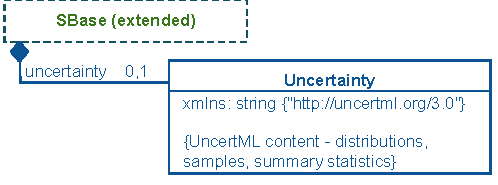
\includegraphics{extended-sbase}
  \caption{The definition of the extended \SBase class to include a new optional \Uncertainty child, which in turn has an \UncertML child in the \uncertml namespace.  Intended for use with any element with mathematical meaning, or with a \Math child.}
  \label{extended-sbase-uml}
\end{figure}

A few SBML elements can interact in interesting ways that can confuse the semantics here.  A \Reaction element and its \KineticLaw child, for example, both reference the exact same mathematics, and should therefore have the same \Uncertainty.  Similarly, if an \InitialAssignment assigns to a constant element (\Parameter, \Species, etc.), the uncertainty for both should be the same, or only one should be provided.

Other elements not listed above should probably not be given an \Uncertainty child, as it would normally not make sense to talk about the uncertainty of something that doesn't have a corresponding mathematical meaning.  However, because packages or annotations can theoretically give new meaning (including mathematical meaning) to elements that previously did not have them, this is not a requirement.


\subsection{The \class{Uncertainty} class}
\label{uncertainty-class}

The \Uncertainty class is a container for \UncertML that descibes the uncertainty in the parent element's mathematical meaning.

The optional \token{id} attribute on the \Uncertainty object class serves to provide a way to identify the uncertainty.  The attribute takes a value of type \primtype{SId}.  Note that the identifier of a the uncertainty carries no mathematical interpretation and cannot be used in mathematical formulas in a model.  \Uncertainty also has an optional \token{name} attribute, of type \primtype{string}.  The \token{name} attribute may be used in the same manner as other \token{name} attributes on \sbmlthreecore objects; please see Section~3.3.2 of the \sbmlthreecore specification for more information.


%It also contains an optional \token{index} attribute:  this is to assist with function definitions that return a vector, and indicate the position in the vector that corresponds to the parent element's value.  For example, a \FunctionDefinition might define an explicit PMF where each realization contains three values, one for each of three different parameters in the model (see example \sec{uncertmath-index-example}).  Each of the three parameters could be given an \Uncertainty child containg \UncertMath referencing that \FunctionDefinition, each with the index of the vector corresponding to its value.  Note that the index is zero-indexed:  the first position in the vector will have an \token{index} of \val{0}, the second of \val{1}, etc.
%
%With the release of the Arrays package, presumably the need for this attribute will go away, but it seems a simple enough addition in the absence of that package, and would provide a tangible benefit to many.  Even after the release of the Arrays package, some software might not support arrays, but will still want to annotate this information:  this attribute will allow them to do so.  See \sec{extended-sbase-examples} for examples of how this might work.


\subsection{The \class{UncertML} class}
\label{uncertml-class}

The \UncertML class is defined as describing the uncertainty in its parent element's mathematics.  It may contain arbitrary \uncertml, which means it has the capability to provide anything from a full distribution to a \token{Sample} element to summary statistics such as \token{StandardDeviation} and \token{Mean}.  There is no requirement that this \uncertml be wrapped in a single element.

For convenience, \uncertml provides a \token{StatisticsCollection}, which may be used to collect multiple other elements.  For clarity, if more than one \uncertml statistics element or \token{StatisticsCollection} are present, they should not conflict with each other.

The namespace for IDs used in the \uncertml is the SId namespace of elements with mathematical meaning in the model, including from other packages.  If that other package is not understood by an interpreter, the \UncertML element may be ignored.  If an interpreter does not understand an ID and cannot tell whether that ID came from a not-understood package, it may issue a warning.


%\subsection{The \class{Math} class}
%\label{uncertmath-class}

%The \UncertMath class child of \Uncertainty, like the \UncertML class, describes the uncertainty in its parent element's mathematics.  It is provided as a way to reference distributions defined in function definitions elsewhere in the model which have been extended by \distribshort.  The most straightforward way to use the \UncertMath class is to simply include a single call to a \FunctionDefinition.  Other uses, such as adding a constant to a function definition (\val{myfunc(3.1) + 2}) are also possible, but discouraged.

%The namespace for IDs used in the \mathml is the SId namespace of elements with mathematical meaning in the model, including from other packages.  If that other package is not understood by an interpreter, the \UncertMath element may be ignored.  If an interpreter does not understand an ID and cannot tell whether that ID came from a not-understood package, it may issue a warning.

%It should be emphasized that this \UncertMath class is \emph{not} intended to be used as a way to explicitly define a probability density function.  Instead, it is a way to provide a \emph{reference} to a PDF or PMF, as defined within an extended \FunctionDefinition.


\subsection{Examples using extended \SBase}
\label{extended-sbase-examples}

Several examples are given to illustrate the use of the \Uncertainty class:


\subsubsection{Basic \UncertML example}

In these examples, a parameter is given an \UncertML child to describe its uncertainty in two ways:


{\color{red}%
Stuart: I'd \controversial give 2 examples here. Although you could put both
constructs together it may confuse to do so as a basic
example. Actually looking at this example I think it would be simpler
to only allow this type of construct for parameters. Here you are
defining the uncertainty about the \emph{initialConcentration} of the
species, not the species itself. For example if you
define the uncertainty, but not the initialConcentration, what does
the uncertainty describe in this case? If you can only describe the
uncertainty of a parameter then this problem does away if the
parameter is used to describe the initial concentration. For example:

\begin{example}
  <parameter id="ic" value="3.22">
    <distrib:uncertainty>
      <uncertml xmlns="http://uncertml.org/3.0">
        <NormalDistribution>
          <mean> ic </mean>
          <variance> 0.09 </variance>
        </NormalDistribution>
      </uncertml>
    <distrib:uncertainty>
  </parameter>
...
  <species id="x" compartment="C" boundaryCondition="false" initialConcentration="ic"
           hasOnlySubstanceUnits="false" constant="false"/>
...
\end{example}

}


\begin{example}
...
  <species id="x" compartment="C" boundaryCondition="false" initialConcentration="3.22"
           hasOnlySubstanceUnits="false" constant="false">
    <distrib:uncertainty>
      <uncertml xmlns="http://uncertml.org/3.0">
        <NormalDistribution>
          <mean> 3.2 </mean>
          <variance> 0.09 </variance>
        </NormalDistribution>
        <StandardDeviation>
          <values> 0.3 </values>
        </StandardDeviation>
      </uncertml>
    <distrib:uncertainty>
  </species>
...
\end{example}

In the above example, a species whose initial concentration is 3.22 is noted as coming from a normal distribution with a mean of 3.2 and a variance of 0.09.  Additionally, its standard deviation is given as 0.3.  In this case, the standard deviation could have been calculated from the variance directly; the modeler has chosen to include both elements for the benefit of any other software that might understand standard deviation, but not the 'distributions' branch of \uncertml.

Note also that 3.22 (the \token{initialConcentration}) is different from 3.2 (the \token{mean}):  evidently, this model was constructed as a realization of the underlying uncertainty, instead of trying to capture the single most likely model of the underlying process.


%\subsubsection{Combining \UncertML and \UncertMath}

%This example is the same as the previous one, but uses \UncertMath to reference a \FunctionDefinition defined as a normal distribution, and \UncertML to note the standard deviation:

%\begin{example}
%...
%<listOfFunctionDefinitions>
%  <functionDefinition id="normal">
%    <math xmlns="http://www.w3.org/1998/Math/MathML">
%      <lambda>
%        <bvar>
%          <ci> mean </ci>
%        </bvar>
%        <bvar>
%          <ci> variance </ci>
%        </bvar>
%        <ci> mean </ci>
%      </lambda>
%    </math>
%    <drawFromDistribution xmlns="http://www.sbml.org/sbml/level3/version1/distrib/version1">
%        <listOfDistribInputs>
%          <distribInput id="avg" index="0"/>
%          <distribInput id="var" index="1"/>
%        </listOfDistribInputs>
%       <uncertml xmlns="http://uncertml.org/3.0">
%         <NormalDistribution>
%           <mean> avg </mean>
%           <variance> var </variance>
%         </NormalDistribution>
%       </uncertml>
%    </drawFromDistribution>
%  </functionDefinition>
%</listOfFunctionDefinitions>
%<listOfSpecies>
%  <species id="x" compartment="C" boundaryCondition="false" initialConcentration="3.22"
%           hasOnlySubstanceUnits="false" constant="false">
%    <distrib:uncertainty>
%      <uncertml xmlns="http://uncertml.org/3.0">
%        <StandardDeviation>
%          <values> 0.3 </values>
%        </StandardDeviation>
%      </uncertml>
%      <math xmlns="http://www.w3.org/1998/Math/MathML">
%        <apply>
%          <ci> normal </ci>
%          <cn> 3.2 </cn>
%          <cn> 0.09 </cn>
%        </apply>
%      </math>
%    <distrib:uncertainty>
%  </species>
%</listOfSpecies>
%...
%\end{example}

%Again, the \UncertML notes that the standard deviation is 0.3, and the \UncertMath notes that the mean is 3.2 and the variance is 0.09.

%\subsubsection{Basic \UncertMath example}

%In the following example, a function definition is created with an \ExplicitPDF child, then used to annotate two parameters.

%\begin{example}
%...
%  <listOfFunctionDefinitions>
%    <functionDefinition id="dist1">
%      <math xmlns="http://www.w3.org/1998/Math/MathML">
%        <lambda>
%          <bvar>
%            <ci> mean </ci>
%          </bvar>
%          <ci> mean </ci>
%        </lambda>
%      </math>
%      <drawFromDistribution xmlns="http://www.sbml.org/sbml/level3/version1/distrib/version1">
%         <listOfDistribInputs>
%           <distribInput id="mean" index="0"/>
%         </listOfDistribInputs>
%         <math xmlns="http://www.w3.org/1998/Math/MathML">
%            <apply>
%              <times/>
%              <apply>
%                <divide/>
%                <cn> 1 </cn>
%                <apply>
%                  <times/>
%                  <cn> 0.011 </cn>
%                  <apply>
%                    <root/>
%                    <degree>
%                      <cn> 2 </cn>
%                    </degree>
%                    <apply>
%                      <times/>
%                      <cn> 2 </cn>
%                      <pi/>
%                    </apply>
%                  </apply>
%                </apply>
%              </apply>
%              <apply>
%                <exp/>
%                <apply>
%                  <times/>
%                  <apply>
%                    <divide/>
%                    <apply>
%                      <power/>
%                      <apply>
%                        <minus/>
%                        <apply>
%                          <minus/>
%                          <ci> x </ci>
%                          <ci> mean </ci>
%                        </apply>
%                      </apply>
%                      <cn> 2 </cn>
%                    </apply>
%                    <cn> 2 </cn>
%                  </apply>
%                  <apply>
%                    <power/>
%                    <cn> 0.011 </cn>
%                    <cn> 2 </cn>
%                  </apply>
%                </apply>
%              </apply>
%            </apply>
%        </math>
%      </drawFromDistribution>
%    </functionDefinition>
%  </listOfFunctionDefinitions>
%  <listOfParameters>
%    <parameter id="y" value="1.1" constant="true">
%      <distrib:uncertainty>
%        <math xmlns="http://www.w3.org/1998/Math/MathML">
%          <apply>
%            <ci> dist1 </ci>
%            <cn> 1.1 </cn>
%          </apply>
%        </math>
%      </distrib:uncertainty>
%    </parameter>
%    <parameter id="z" value="3.2" constant="true">
%      <distrib:uncertainty>
%        <math xmlns="http://www.w3.org/1998/Math/MathML">
%          <apply>
%            <ci> dist1 </ci>
%            <cn> 3.2 </cn>
%          </apply>
%        </math>
%      </distrib:uncertainty>
%    </parameter>
%  </listOfParameters>
%...
%\end{example}

%In the above example, a function definition is provided with an \ExplicitPDF that defines a distribution with a mean of \val{mean} and a variance of \val{0.011}.  The parameters \val{y} and \val{z} are each annotated with an \UncertMath child that calls that function, the first with the argument \val{1.1} (its value), and the second with the argument \val{3.2} (its value).  The effect of adding the \Uncertainty children, then, is to denote that both values come from a gaussian distribution with a mean of the parameter value, and a variance of \token{0.011}.  Note that this use of the \distribshort package does not use \uncertml at all.

\subsubsection{Defining a Random Variable}

In addition to describing the uncertainty about an experimental
observation one can also use this mechanism to describe a parameter as
a random variable. In the example below the parameter, $Z$, is defined
as following a normal distribution, with a given mean and variance. No
value is given for the parameter so it is then up the modeller to
decide how to use this random variable. For example they may choose to
simulate the model in which case they may provide values for $mu\_Z$
and $var\_Z$ and then sample a random value from the
simulation. Alternatively they may choose to carry out a parameter
estimation and use experimental observations to estimate $mu\_Z$ and
$var\_Z$.

\begin{example}
    <listOfParameters>
	<parameter id=”mu_Z” value=”10”/>
	<parameter id=”var_Z value=”0.1”/>
	<parameter id="Z">
          <distrib:uncertainty>
	    <Distribution  xmlns="http://www.uncertml.org/3.0">
	      <NormalDistribution>
	        <mean><ref id="mu_Z"/></mean>
	        <variance><ref id=”var_Z”/></variance>
	      </NormalDistribution>
	    </Distribution>
          </distrib:uncertainty>
	</parameter>
    </listOfParameters>   
\end{example}

{\color{red}%
  Stuart:\controversial This example illustrates the kind of use cases
  I was describing at HARMONY. I hope this isn't controversial, but I
  want us to be clear that we all happy using this interpretation of
  uncertainty too. If so then it makes sense to have an example. }

{\color{red}%
  Stuart:\controversial In writing this I just realised that you are
  using an <uncertml xmlns="http://uncertml.org/3.0"> element to
  define uncertml elements. I know there is a whole section devoted to
  it, but I didn't realise the significance of it. In \uncertml there
  isn't an element like this. In \uncertml 3.0 the plan is to provide
  3 grouping elements for each of the subsets in \uncertml:
  Statistics, Distributions and Samples. The idea behind this is it
  allows an XML language that uses \uncertml to constrain its use to
  one or more of these subsets. So for example if we only want to use
  distributions then we only allow an \uncertml Distribution element
  at a given point. This is shown in the example above. I haven't
  changed any of the other examples or the class diagrams, but I think
  they do need to be modified accordingly.
}


\subsubsection{An \UncertML example with a PMF}
\label{uncertmath-index-example}

In the following example, a species and two parameters are all given \UncertML children indicating that they were sampled from a PMF.  Because all three have the same \token{Realisation} IDs, the assumption can be made that the three values are correlated, and are drawn from \val{patient1}, \val{patient2}, or \val{patient3}.

\begin{example}
...
  <listOfSpecies>
    <species id="S1" compartment="C" boundaryCondition="false" initialConcentration="2.24"
             hasOnlySubstanceUnits="false" constant="false">
      <distrib:uncertainty>
         <uncertml xmlns="http://uncertml.org/3.0">
           <UnknownSample>
             <Realisation id="patient1">
               <weight> 0.5 </weight>
               <values> 1.01 </values>
             </Realisation>
             <Realisation id="patient2">
               <weight> 0.25 </weight>
               <values> 2.24 </values>
             </Realisation>
             <Realisation id="patient3">
               <weight> 0.25 </weight>
               <values> 1.72 </values>
             </Realisation>
           </UnknownSample>
         </uncertml>
      </distrib:uncertainty>
    </species>
  </listOfSpecies>
  <listOfParameters>
    <parameter id="y" constant="true" value="45.9">
      <distrib:uncertainty>
         <uncertml xmlns="http://uncertml.org/3.0">
           <UnknownSample>
             <Realisation id="patient1">
               <weight> 0.5 </weight>
               <values> 42.3 </values>
             </Realisation>
             <Realisation id="patient2">
               <weight> 0.25 </weight>
               <values> 45.9 </values>
             </Realisation>
             <Realisation id="patient3">
               <weight> 0.25 </weight>
               <values> 50.0 </values>
             </Realisation>
           </UnknownSample>
         </uncertml>
      </distrib:uncertainty>
    </parameter>
    <parameter id="z" constant="true" value="0.002">
      <distrib:uncertainty>
         <uncertml xmlns="http://uncertml.org/3.0">
           <UnknownSample>
             <Realisation id="patient1">
               <weight> 0.5 </weight>
               <values> 0.004 </values>
             </Realisation>
             <Realisation id="patient2">
               <weight> 0.25 </weight>
               <values> 0.002 </values>
             </Realisation>
             <Realisation id="patient3">
               <weight> 0.25 </weight>
               <values> 0.0033 </values>
             </Realisation>
           </UnknownSample>
         </uncertml>
      </distrib:uncertainty>
    </parameter>
  </listOfParameters>
...
\end{example}

In this example, the chosen value for all three elements is the Realisation from \val{patient2}, and presumably comes from the same external data source.

{\color{red} Stuart:\controversial I'm not at all sure about this. I
  don't think that's a correct use of realisations to interpret that the same ID implies correlation. However, I have asked Dan
  for clarification on the use of realisations so we can get the
  definitive view on this. Aside from the above example it may be good
  to start off with a simple example. How about this?

\begin{example}
...
  <parameter id="gender">
    <distrib:uncertainty>
      <Statistic  xmlns="http://www.uncertml.org/3.0">
        <DiscreteProbability>
          <!-- M=0 F=1 -->
          <categories>0 1</mean>
          <probabilities>0.6 0.4</probabilities>
        </DiscreteProbability>
      </Statistic>
    </distrib:uncertainty>
  </parameter>
...
\end{example}

We could be clever and add a third gender!
}

In a version of this model that used Arrays package constructs, a single vector could be created with all three values in it, and given an \UncertML child with \token{value} elements that contained vectors instead of single values.


\section{Interaction with other packages}

This package is dependent on no other package, but relies on the \arrays package
to provide vector and matrix structures if those are desired/used.

If the \req package is used, any \FunctionDefinition that has been given an \DrawFromDistribution child must be given a \ChangedMath child referencing this package's namespace.  If the fallback function provides a complete \LambdaClass function, its \token{viableWithoutChange} atribute \emph{may} be set \val{true} if the modeler considers that function an acceptable alternative to the draw from the distribution, otherwise it must be set \val{false}.



\section{Use-cases and examples}

The following examples are more fleshed out than the ones in the main text, and/or illustrate features of this package that were not previously illustrated.

\subsection{Sampling from a distribution: PK/PD Model}

This is a very straightforward use of an \uncertml-defined
distribution. The key point to note is that a value is sampled from
the distribution and assigned to a variable when it is invoked in the
initialAssignments element in this example. Later use of the variable
does not result in re-sampling from the distribution. This is
consistent with current SBML semantics.

{\color{red}Stuart:\controversial I'd like to add another example here
  that defines them model without sampling. We can have 2 versions of
  the same model. I'll come back to it...}

\exampleFile{examples/pkpd.xml}


\subsection{Truncated distribution}
\label{sec: truncated-eg}

To encode a truncated distribution we rely on an as-of-this-writing hypothetical extention to \uncertml (the \token{lower} and \token{upper} child elements of \token{NormalDistribution}).  The final version of truncation in \uncertml may not look exactly like this example, but should follow the basics.  Note that the values for truncation are here provided as arguments to the function definition, but could instead be hard-coded.

\exampleFile{examples/truncated_distn.xml}


\subsection{Multivariate distribution}

In this example two correlated parameters are sampled from a
multivariate distribution. The correlation is defined using a
covariance matrix and the sampled values are returned as a vector of 2
values, and assigned to the variable \val{correlated\_params}.  This vector is then used to assign values to \val{V} and \val{C1}, thereby associating those two values with the same draw from the multivariate normal distribution.  The use of various array and matrix \mathml here is speculative:  in the absence of a finalized Arrays package, it is impossible to tell exactly what form that will take.  However, all of the functionality expressed here will need to be incorported in some form into the Arrays package, and much if not all of it may take the form illustrated here.

\exampleFile{examples/mutivariate_example.xml}


\subsection{User-defined continuous distribution }

In this example, an extended function definition is constructed, and used in three places:  to denote the uncertainty in the parameter \val{V}, the uncertainty in the initial assignment to \val{V}, and to construct the initial assignment itself.  Note that strictly speaking, since \val{V} is constant, one could assume that the uncertainty in the parameter itself was identical to the uncertainty in its initial assigment; both are given here by way of illustration.

{\color{red}Stuart:\controversial I don't understand how this is a
  user-defined continuous distribution. It's just showing the usage of
  a distribution. No?
}

\exampleFile{examples/user-defined.xml}


\subsection{User-defined discrete distribution}
\label{sec:userDefinedDiscrete}

In this example, a \DistributionOrSample is used where the weights themselves are the arguments to the function instead of the values.

\exampleFile{examples/user-defined-pmf.xml}


\section{Prototype implementations}

None as yet.


\section{Unresolved issues}
\label{sec:unresolved}


{\color{red} Stuart:\controversial I'm happy to removed this section -
  unless of course any new issues come up!}

\begin{enumerate}
\item Should the ExplicitPDF class have a truncation
  attribute? This would allow one to define a truncated distribution
  without defining the truncated PDF in the \mathml definition. Is
  this desirable or not?
  \emph{Lucian:  I think not.  Since explicit PDFs can already be truncated through the use of the 'piecewise' function, let's see how this works out for people first before putting in new functionality that has to be implemented explicitly.  (On the other hand, it may turn out that if people have to implement it for UncertML, they may not mind implementing it for explicit PDFs either.  In that case if it was much easier to implement truncated explicit PDFs as models, it might be worth adding in some constructs.  Either way, I vote for waiting for implementations to clear things up here.)}
  \emph{Lucian: Follow-up:  Explicit PDFs have been removed entirely!}

\item Currently the proposal provides an appendix that clarifies the
  parameters that should be specified for each \uncertml distribution and their
  type. It also defines whether one or more values are sampled from a
  given distribution. There was some argument on the list about
  whether this appendix is required. An alternative would be to use
  \uncertml definitions as-is, and live with any inherent
  ambiguity. We should make a decision about the approach we want to
  take for the final version of this proposal.
  \emph{Lucian:  As is obvious, we did indeed go with using the uncertML as-is.  I think it works out a lot better this way, though I would still keep the appendix to ensure people understand the different distributions.}

\item The use of arrays. The package and examples have been written
  that some distribution definitions will require the use of vector or
  matrix types that can be provided by the Arrays package. While
  relying on such types enables us to describe a wide range of
  probability distributions this will come at the cost of delaying
  this package's approval until Arrays has been developed and
  approved. There are two alternative strategies. One is to only
  support distributions that do not require array types (see appendix
  \ref{sec:uncertmlusage}). The other would be to define workarounds
  within \distribshort to provide array structures without using the
  arrays package. The decision at COMBINE was to wait. Do we want to
  revisit this decision?
  \emph{Lucian:  I tried to write this specification in such a way that when Arrays is available, it will work seamlessly with distrib, and until that time, everything that does *not* require Arrays will still work.  This will also allow people to implement support for each separately.}

\item Currently sampling of distributions in permitted in the event
  related elements of SBML: EventAssignments, Delays and
  Priorities. The reason for prohibiting sampling in a rate law (or other
  circumstances where the model is being continuously evaluated) was
  because this can make the simulation unstable\footnote{See slide entitled Extrinsic
  noise:
  \url{http://sbml.org/images/3/3b/Djw-sbml-hackathon-2010-05-04.pdf}.}. It
  is unclear whether a similar situation could arise while sampling from
  events. The author feels this need to be looked into further by 'who
  know'.
  \emph{Lucian:  I believe this has been resolved.}

\item During the review of this proposal it was questioned whether the
  use of the term PMF was appropriate for the eponymous \distribshort
  class: \class{userDefinedPMF}. The issue is that a PMF is defined
  for (numerical) values which a random variable can assume and not
  general 'categories'. Since we permit non-numerical values to define
  categories such as eye colour (red, green, blue etc.) or sex (M, F)
  it is argued that the current name is mis-leading. \uncertml uses
  the term discrete probability for a similar construct that describes
  this, so perhaps a better class name would be
  \class{UserDefinedDiscreteProbability} or just
  \class{DiscreteProbability}.
  \emph{Lucian:  There was a bit of discussion on the list in favor of 'PMF'; I have retained that wording in this version.}

\item Limiting the use of \class{FunctionDefinition}. In review it was
  pointed out that the restriction on sampling to InitialAssignent,
  EventAssignment etc. affects MathML validity rules in SBML. Currently
  a function definition can be 'called' from any \mathml block in an
  SBML document. However, \distribshort imposes an additional special
  case. \emph{A function definition that defines a distribution can
    only be called from \mathml, where sampling is permitted.} It is
  not absolutely clear what the technical implications of this are,
  but it would appear that to implement \distribshort support any
  implementation would be required to modify the \mathml validation
  rules in libSBML. Given, that these rules are not designed to
  interact with packages this may be technically challenging to
  implement. The author feels that it would be desirable to find an
  alternative design that avoids the need to modify the \mathml
  validation rules.
  \emph{Lucian:  This was the main topic of discussion on the list, and the result of the survey that we put out at the end was that we should indeed continue to extend FunctionDefinitions, but should *not* limit their use to discrete contexts.  Rather, to allow 'continuous' contexts to work in the future, they should be allowed but their behavior now should be undefined, and their use discouraged.  That is the tack I have tried to take in this version of the document.}
\end{enumerate}

\section{Acknowledgements}
\label{sec:acknowledgements}

Much of the initial concrete work leading to this proposal document
was carried out at the Statistical Models Workshop in Hinxton in 2011,
which was organised by Nicolas le Nov\`{e}re. A list of participants
and recordings of the discussion is available from
\url{http://sbml.org/Events/Other_Events/statistical_models_workshop_2011}.
Before that a lot of the ground work was carried out by Darren
Wilkinson who led the discussion on \distribshort at the Seattle SBML
Hackathon and before that Colin Gillespie who wrote an initial
proposal back in 2005. The author would also like to thank the
participants of the \distribshort sessions during HARMONY 2012 and
COMBINE 2012 for their excellent contributions in helping revising
this proposal; Sarah Keating, Maciej Swat and Nicolas le Nov\`{e}re
for useful discussions, corrections and review comments; and Mike
Hucka for \LaTeX{} advice and the beautiful template upon which this
document is based.

\appendix
\section{Changes anticipated in UncertML 3.0}

{\color{red}Stuart:\controversial Add a section here or in the main text outlining what
  UncertML 3.0 will look like.}

\bibliography{sbml-level-3-distrib-package-proposal}


\end{document}

